\documentclass[10pt,twocolumn,letterpaper]{article}

\usepackage{cvpr}
\usepackage{times}
\usepackage{epsfig}
\usepackage{graphicx}
\usepackage{amsmath}
\usepackage{amssymb}

% Include other packages here, before hyperref.
\usepackage{graphicx}

% If you comment hyperref and then uncomment it, you should delete
% egpaper.aux before re-running latex.  (Or just hit 'q' on the first latex
% run, let it finish, and you should be clear).
\usepackage[breaklinks=true,bookmarks=false]{hyperref}

\cvprfinalcopy % *** Uncomment this line for the final submission

%\def\cvprPaperID{****} % *** Enter the CVPR Paper ID here
\def\httilde{\mbox{\tt\raisebox{-.5ex}{\symbol{126}}}}

% Pages are numbered in submission mode, and unnumbered in camera-ready
%\ifcvprfinal\pagestyle{empty}\fi
\setcounter{page}{1}
\begin{document}

%%%%%%%%% TITLE
\title{3D Cross-modal Retrieval: Bridging the Gap between 3D Objects and Natural Language Descriptions}

\author{Nick Harmening\\
Technical University Munich\\
%Arcisstrasse 21, 80333 Munich\\
{\tt\small n.harmening@tum.de}
% For a paper whose authors are all at the same institution,
% omit the following lines up until the closing ``}''.
% Additional authors and addresses can be added with ``\and'',
% just like the second author.
% To save space, use either the email address or home page, not both
\and
Fabian Schramm\\
Technical University Munich\\
%Arcisstrasse 21, 80333 Munich\\
{\tt\small fabian.schramm@tum.de}
}

\maketitle
%\thispagestyle{empty}

%%%%%%%%% ABSTRACT
\begin{abstract}
   We present a method for cross-modal retrieval based on colored point clouds of 3D objects and corresponding natural freeform text descriptions. For said purpose, a Siamese neural network including a triplet loss is used and an advanced architecture with text and shape autoencoders could further improve the retrieval performance. The goal of the network is to construct a meaningful embedding space where corresponding 3D shapes and text descriptions are mapped close together. An user's input query as freeform text can therefore retrieve the best corresponding 3D shape.
\end{abstract}

%%%%%%%%% BODY TEXT
\section{Introduction}

In human cognition visual and auditory impulses are strongly connected and correlated. Language is used to communicate, describe our environment and convey meaningful messages. The visual modality perceives our surroundings and helps to interpret it. In recent years, there were lot of new developments in the field of computer vision and natural language processing. Both fields separately experienced a remarkable boost by the fast development of deep neural networks and new methods proposed currently. Our approach aims at bridging the gap between the two modalities of 3d shapes and natural text descriptions and hereby improve the performance of 3D shape retrieval.
\begin{figure}[h]%[!htbp]
	\centering
	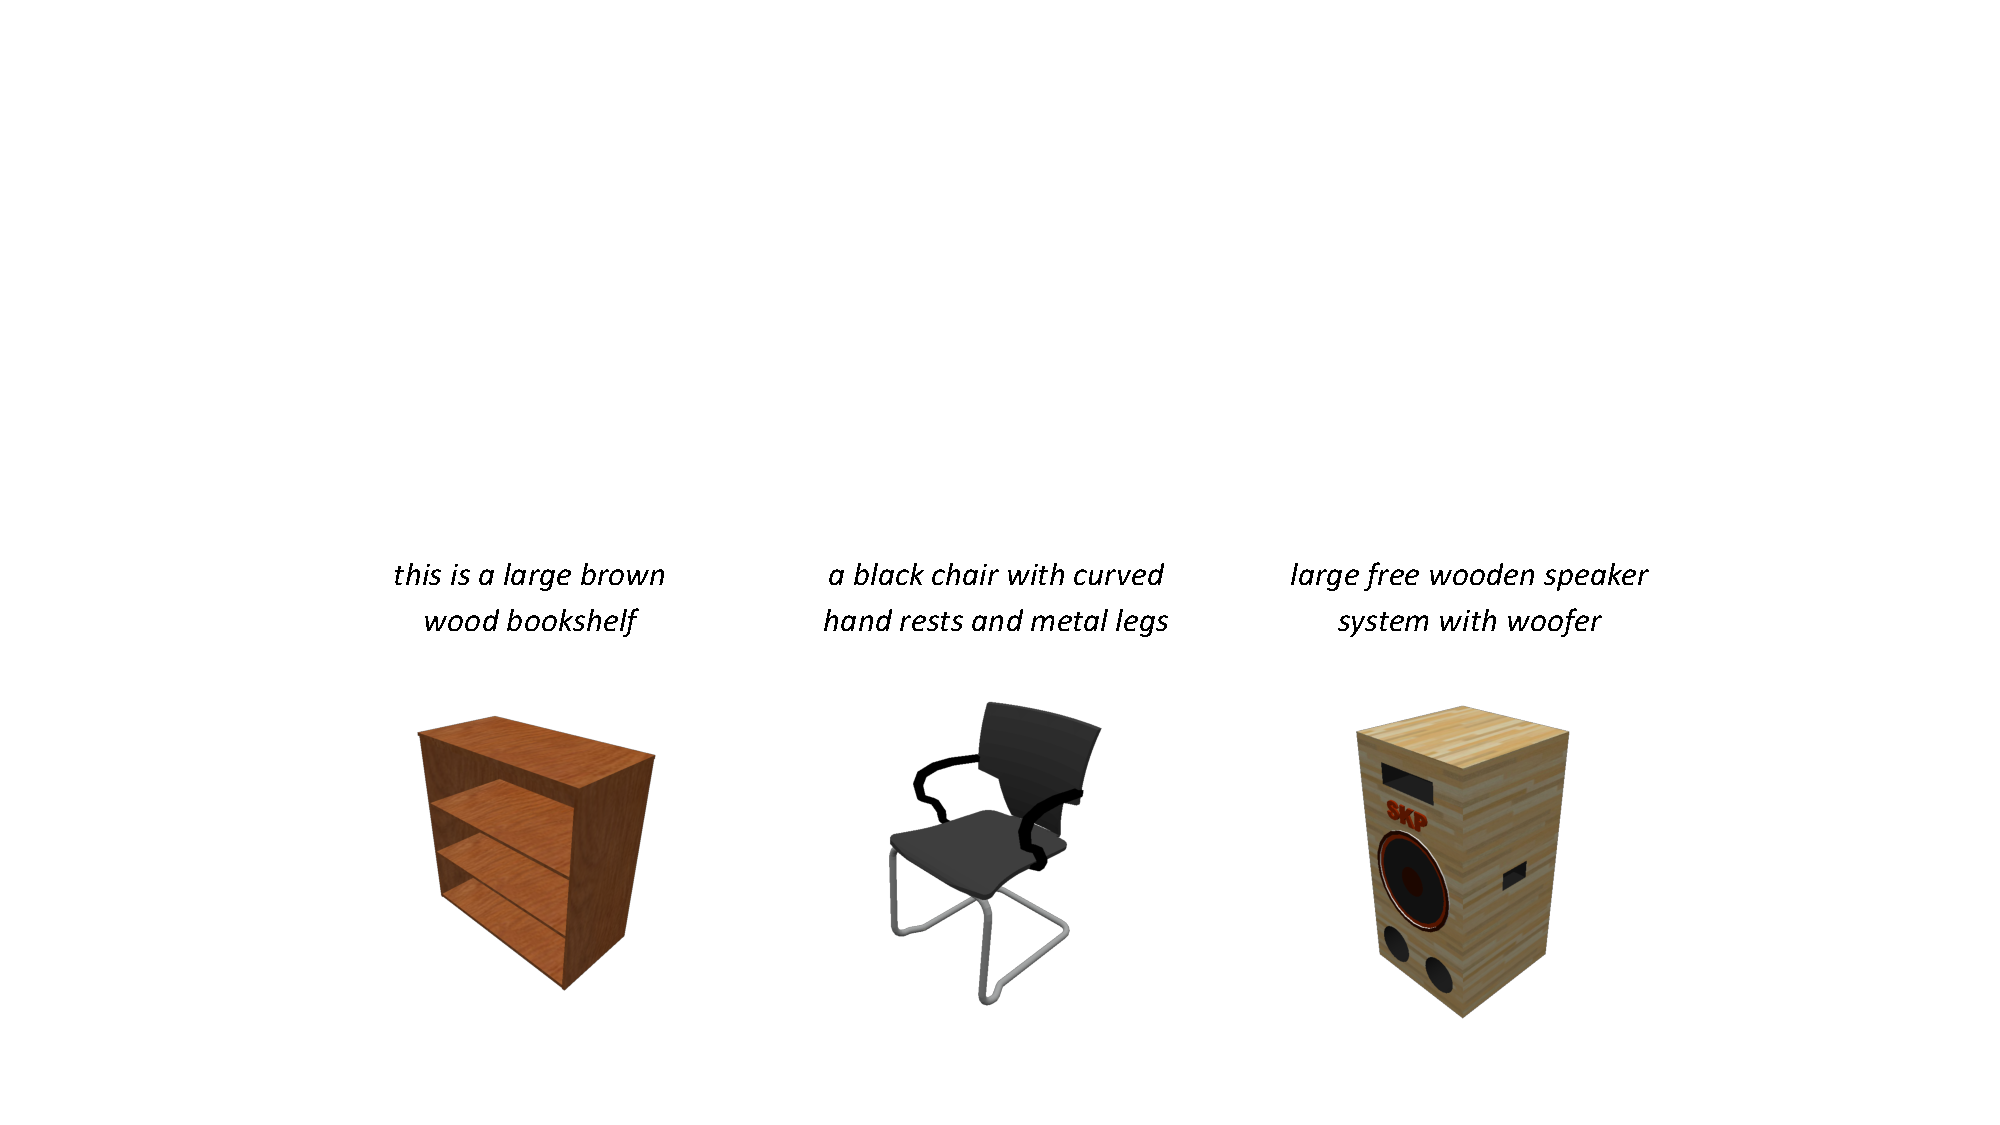
\includegraphics[width=0.8\linewidth]{fig1.pdf}
	\caption[]{Examples of three different instances and each represented in two modalities}
	\label{fig:examples}
\end{figure}
\autoref{fig:examples} depicts two ways of describing the same instance in different modalities, \eg the leftmost instances is a wooden bookshelf. In order to convey the context of said instance, either a natural language description or a colored 3D shape could be used. Combining both information and connecting the context from text and shape allows humans to infer more details about an instance. The goal for the network we develop is the understand the context of the natural language description, of the 3D shape in form of a point cloud and map both into one combined embedding space were corresponding text and shape are close together. This embedding space can be used after training for an user to input a text query and retrieve a corresponding 3D shape or vice versa. The training of shape and text encoding of our network is jointly in an end-to-end fashion. 

\section{Related Work}
There is some work in the field of cross-modal retrieval and representation which we present in the following. To the best of our knowledge, there is no approach on that field which works with a point cloud representation of the 3D shapes. 
Chen \etal \cite{chen2018text2shape} use voxelized 3D shapes and natural language descriptions as input to their network in order to learn joint embeddings. Their models combines learning by association and metric learning approaches and is able to capture implicit cross-modal connections. A round trip loss is introduced and further tasks like generating colored 3D shapes from text is performed. In contrast, the focus of our work is only the 3D shape retrieval and most important our approach is based on point clouds instead of voxels. 

Han \etal \cite{han2018seq2seq} propose a view-based model to learn cross-modal representations by joint reconstruction and prediction of view and word sequence. They thereby overcome the issue of lacking detailed geometry information of the 3D shapes. Again, 3D voxels are used to represent a 3D object and therefore differing from our method.  

Qi \etal developed a deep neural network called PointNet \cite{qi2017pointnet} to perform classification and semantic segmentation with point clouds. The network is designed to directly consume an unordered point cloud as input, without converting it to other 3D representations such as voxel grids first. Additionally, they introduce Pointnet++ \cite{qi2017Pointnet++} which is a hierarchical application of PointNet to capture local context. PointNet++ achieves better performance and generalizability in complex scenes and is able to deal with non-uniform sampling density. A combination of different modalities is not content of these works. 

\section{Dataset}
Our method is learning a joint embedding of freeform text descriptions and 3D shapes. To train and evaluate the model we use the ShapeNet \cite{Chang2015Shapenet} dataset, which is a collecting of human-designed 3D CAD objects. We use 13 categories of the ShapeNetCore Dataset, which is a subset of the full ShapeNet dataset with single clean 3D models and manually verified category and alignment annotations. In total there are around 27,000 objects. Additionally, we there exist five natural language descriptions per 3D object. The 3D shapes are represented as colored meshes in the \textit{obj} file format and a \textit{mat} material file which partly also possess a texture.

The first task of our data pre-processing pipeline is a conversion and sampling step from said meshes, which are stored as vertices and faces, into 3D point clouds of selectable number of points. The appearance of an original 3D CAD model and of resulting point clouds with different numbers of sampling points can be seen in \autoref{fig:sampling}.
\begin{figure}[t]%[!htbp]
	\centering
	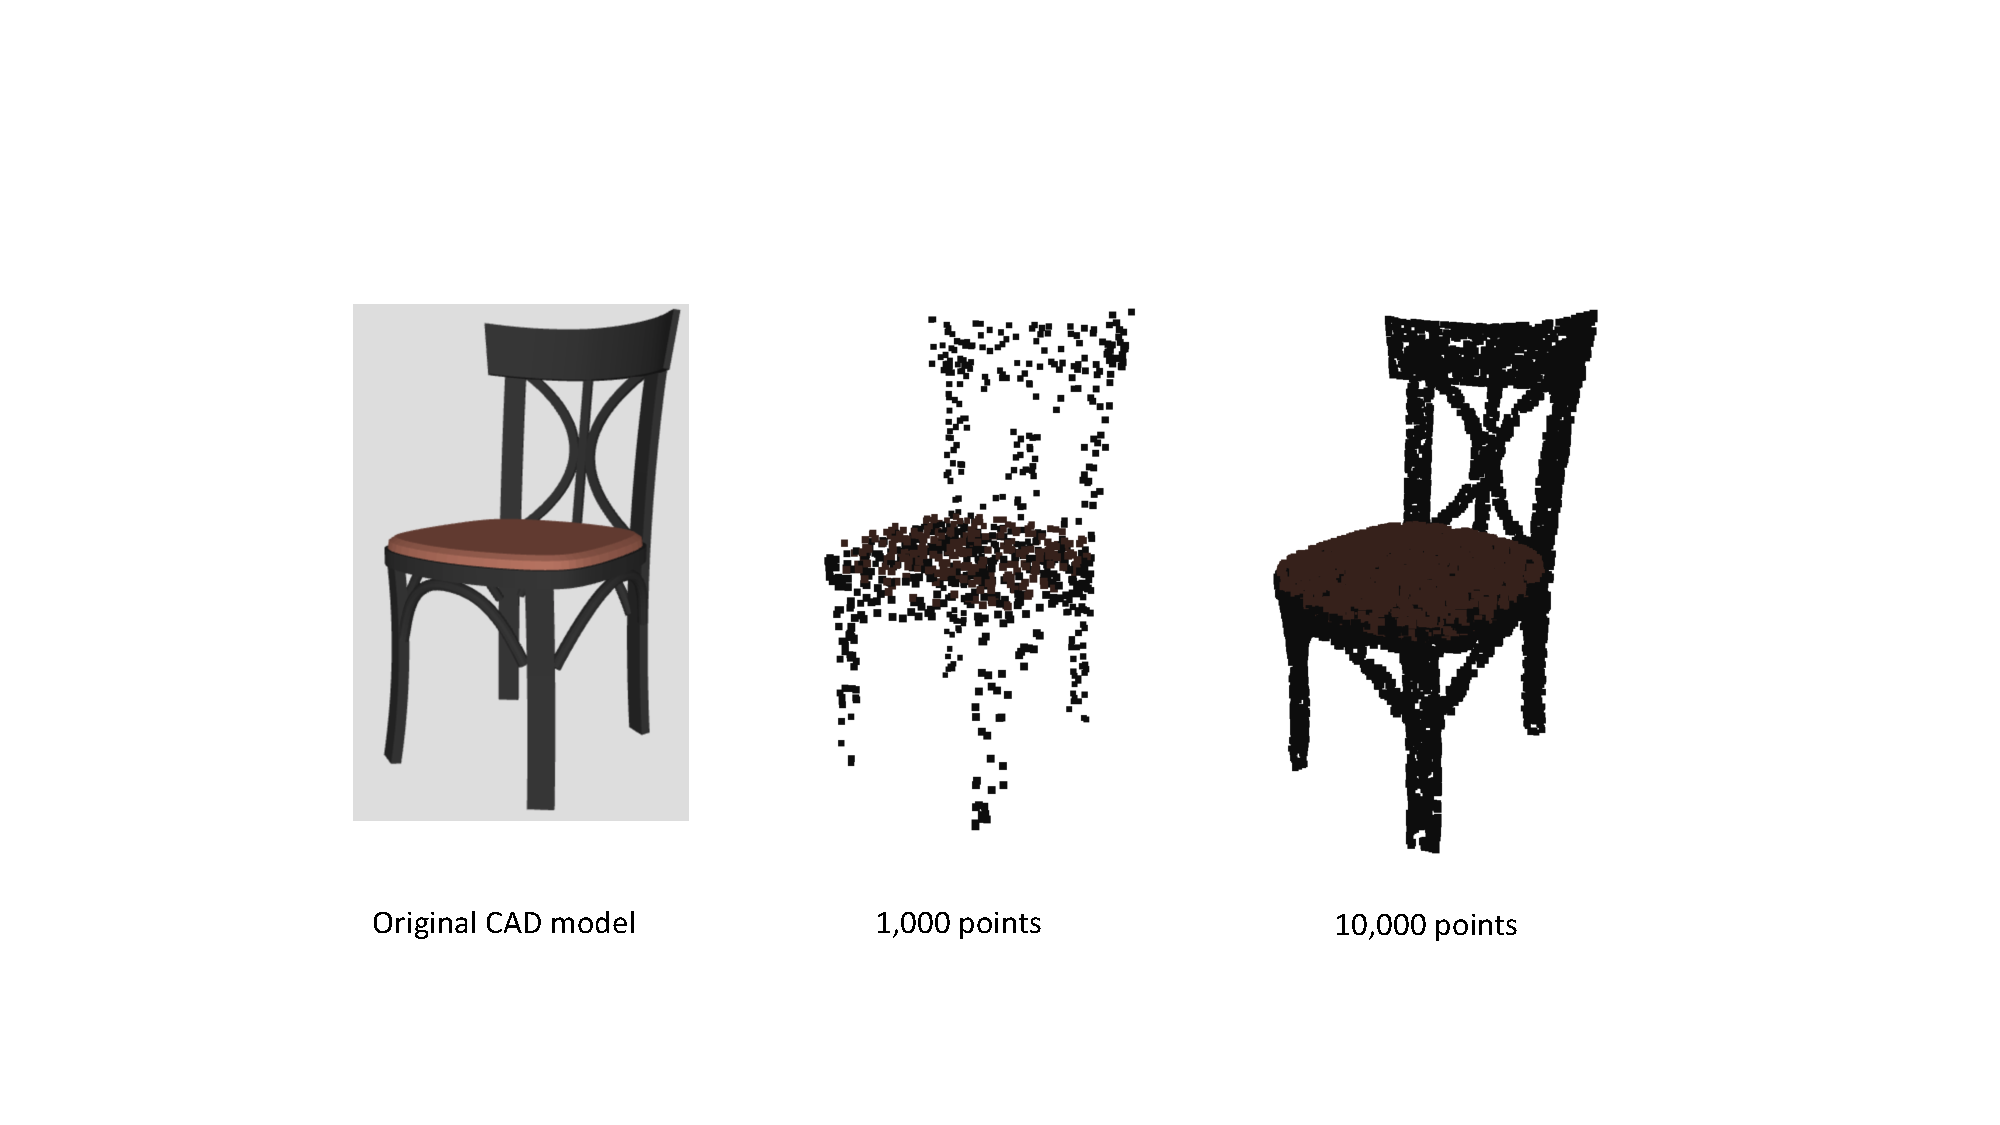
\includegraphics[width=0.8\linewidth]{fig2.pdf}
	\caption[]{3D point cloud sampling from CAD model with different numbers of sample points}
	\label{fig:sampling}
\end{figure}
Denote that a representation of only 1,000 points is quite sparse, whereas 10,000 sampling points are a very dense point cloud. As one of the reasons why we use point clouds is to be remarkable faster and light-weighter than a dense voxel representation, we decided to work with 2000 sampling points. 

The descriptions for the 3D CAD models were collected in a crowed-sourcing process and contain spelling mistakes and grammatical errors. We clean the descriptions by using the \textit{LanguageTool} \footnote{https://languagetool.org}, split the sentence into tokens and discard low frequent words with less than three occurrences. By doing, so we obtain a vocabulary size of 5197 words. All sentences that we provide to our text encoder should be of the same size and therefor we analyzed the descriptions length. The average length of the around 14,000 descriptions is 12.4 words and by cutting every description which is longer than 20 words we still maintain 89\% of all descriptions completely. All descriptions shorter than 20 words are padded with zeros. The natural language words are each converted into arrays of 50 float numbers by using the pre-trained word embedding GloVe \cite{pennington2014glove} in the version \textit{Wikipedia 2014 + Gigaword 5} containing 6B tokens and 400K words. When searching the matching GloVe embeddings for our vocabulary, we end up with 5105 unique word embedding vectors.

\section{Method}
We use a Siamese neural network with a text and shape decoder which are mapping to the same joint embedding space of size $\mathbb{R}^{128}$. In that space, the goal is to keep corresponding text and shape embeddings close together and separate text and shape embeddings of different instances. For that purpose, a triplet loss with margin is used whereby the anchor can either by a shape or a text. 
\subsection{Baseline -- Cross-Modal Siamese}
\begin{figure}[t]%[!htbp]
	\centering
	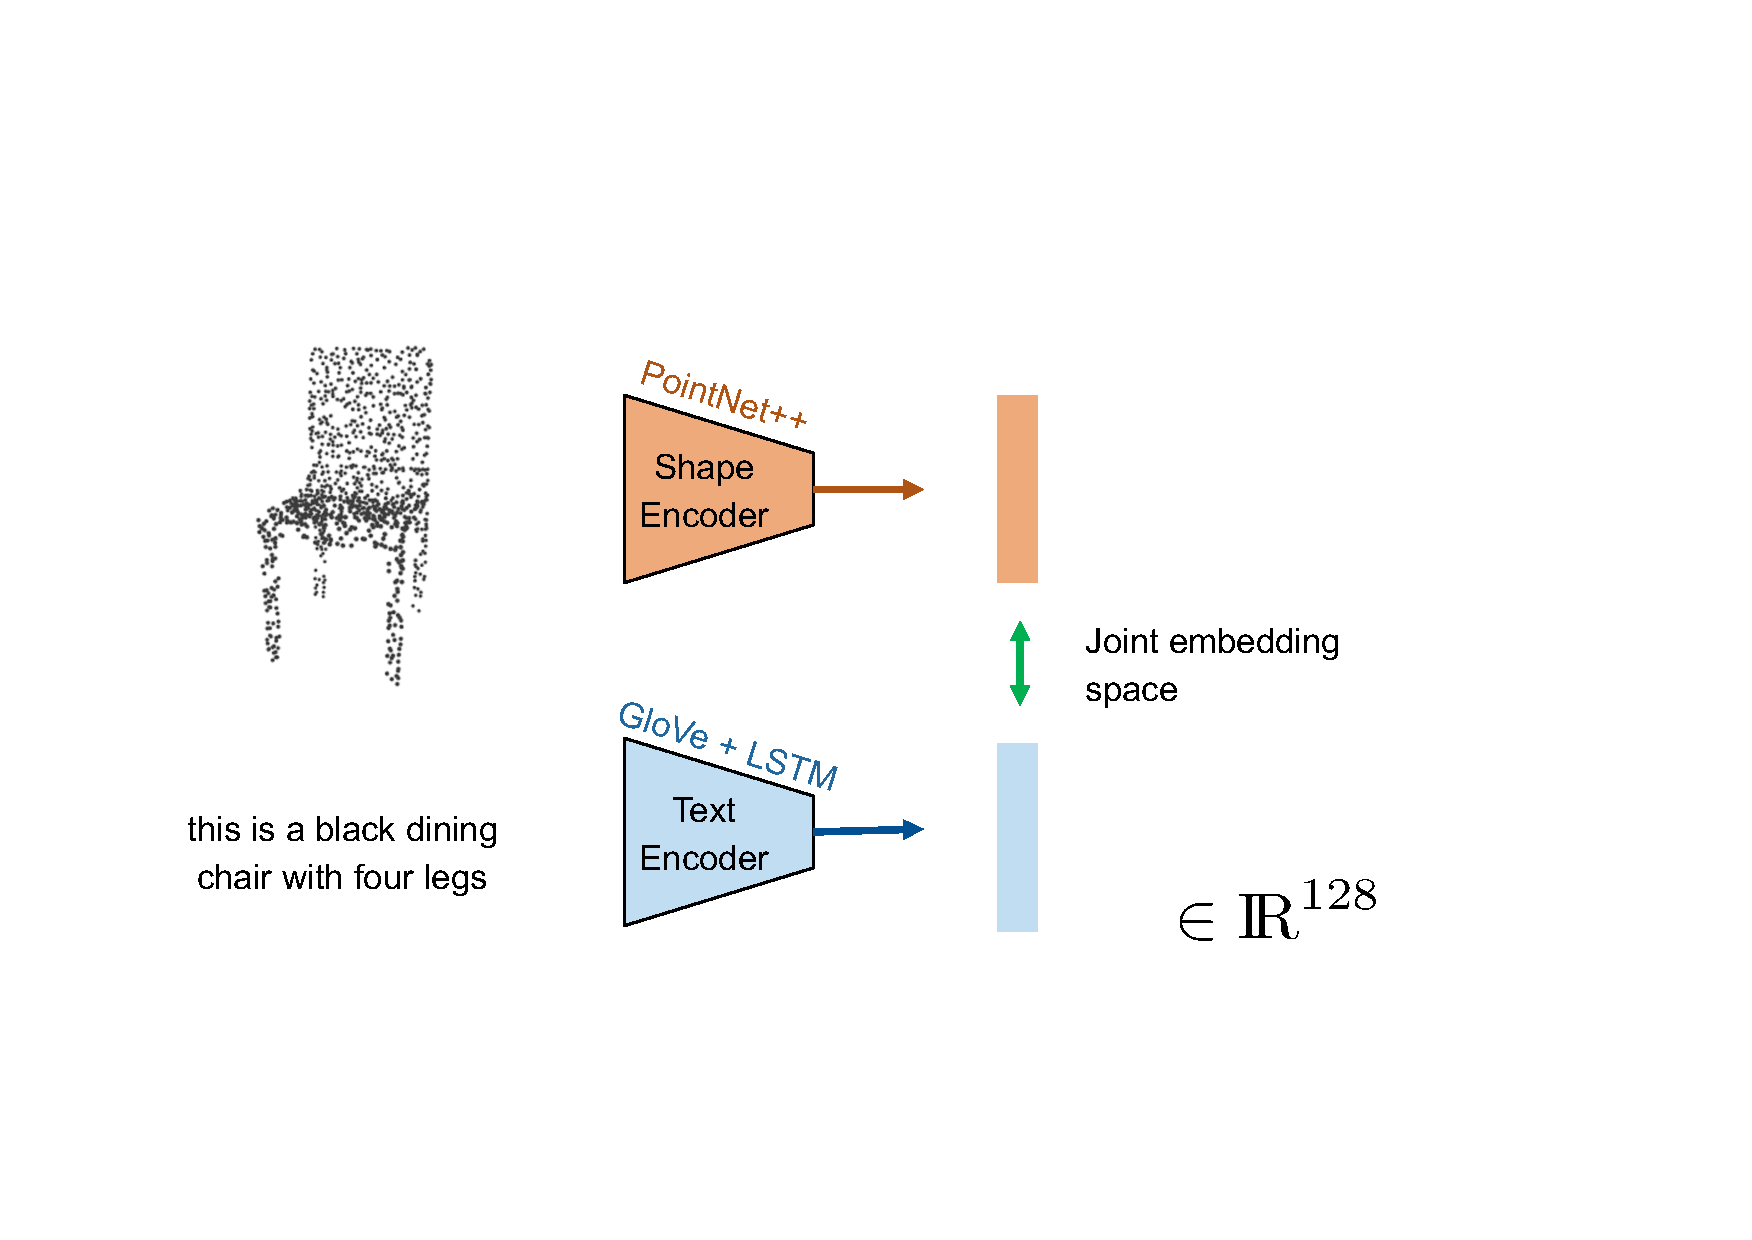
\includegraphics[width=0.8\linewidth]{fig3.pdf}
	\caption[]{Our baseline model consisting of text and shape decoder}
	\label{fig:baseline}
\end{figure}
The baseline configuration of our model is shown in \autoref{fig:baseline} and visualizes the process from 3D shape and text description to embedding of size $\mathbb{R}^{128}$. The text encoder is a two-layer LSTM to capture the temporal information of the description with a fully-connected layer at the end to project in the space $\mathbb{R}^{128}$ and as shape encoder we use a slightly adapted version of PointNett++ \cite{qi2017Pointnet++}. This networks allows to directly consume on 3D point clouds where as additional feature we add the RGB color values of each point. The colored point clouds are projected into the $\mathbb{R}^{128}$ space and compared to the text embeddings using a triplet loss. A formulation of the loss is as follows:
\begin{equation}
\label{eqn:1}
\mathcal{L}_{baseline} = \mathcal{L}_{1} + \mathcal{L}_{2}
\end{equation}
As denoted in eqn. (\ref{eqn:1}), we combine two triplet losses to the final baseline loss. First, we define a shape as an anchor $A^S$ and therefore one text embedding as positive $P^S$, obtained from one of the five descriptions of the shape, and one text embedding as negative $N^T$, obtained from a shape different to the anchor (eqn. (\ref{eqn:2})). The second part of the baseline loss uses one of the five descriptions of an instances as an anchor and therefore the corresponding shape as positive and one other shape as negative (eqn.(\ref{eqn:3})). A margin $m$ is added in order to force a certain distance between anchor-positive and anchor-negative and saturating afterwards. 
\begin{equation}
	\label{eqn:2}
	\resizebox{.9 \linewidth}{!}
	{ $
	\mathcal{L}_1(A^S, P^T, N^T) = \max \left( 0, \left\Vert A^S - P^T\right\Vert^2 - \left\Vert A^S - N^T\right\Vert^2 +m \right) $}
\end{equation}
\begin{equation}
\label{eqn:3}
\resizebox{.9 \linewidth}{!}
{ $
	\mathcal{L}_2(A^T, P^S, N^S) = \max \left( 0, \left\Vert A^T - P^S\right\Vert^2 - \left\Vert A^T - N^S\right\Vert^2 +m \right) $}
\end{equation}
By using this baseline model we are able to project both shape and text into the embedding space in a meaningful way by reducing to triplet loss (eqn.(\ref{eqn:1})). As the triplet loss combines parts of different modalities it enforces to learn a cross-modal connection for the instances. Tp further improve the embedding space and retrieval performance a more sophisticated architectures is presented in the following.

\subsection{Cross-Modal Siamese Autoencoder}
The basic network architectures is similar to our baseline, mapping into the embedding space $\mathbb{R}^{128}$ with a LSTM for the text descriptions, PointNet++ for the shapes and evaluating it by a triplet loss. Additionally, we add a text and shape decoder into our pipeline which project the embeddings again up into a higher dimensional space, where they are compared to the original inputs. The new setting is depicted in \autoref{fig:autoencoder}.
\begin{figure}[t]%[!htbp]
	\centering
	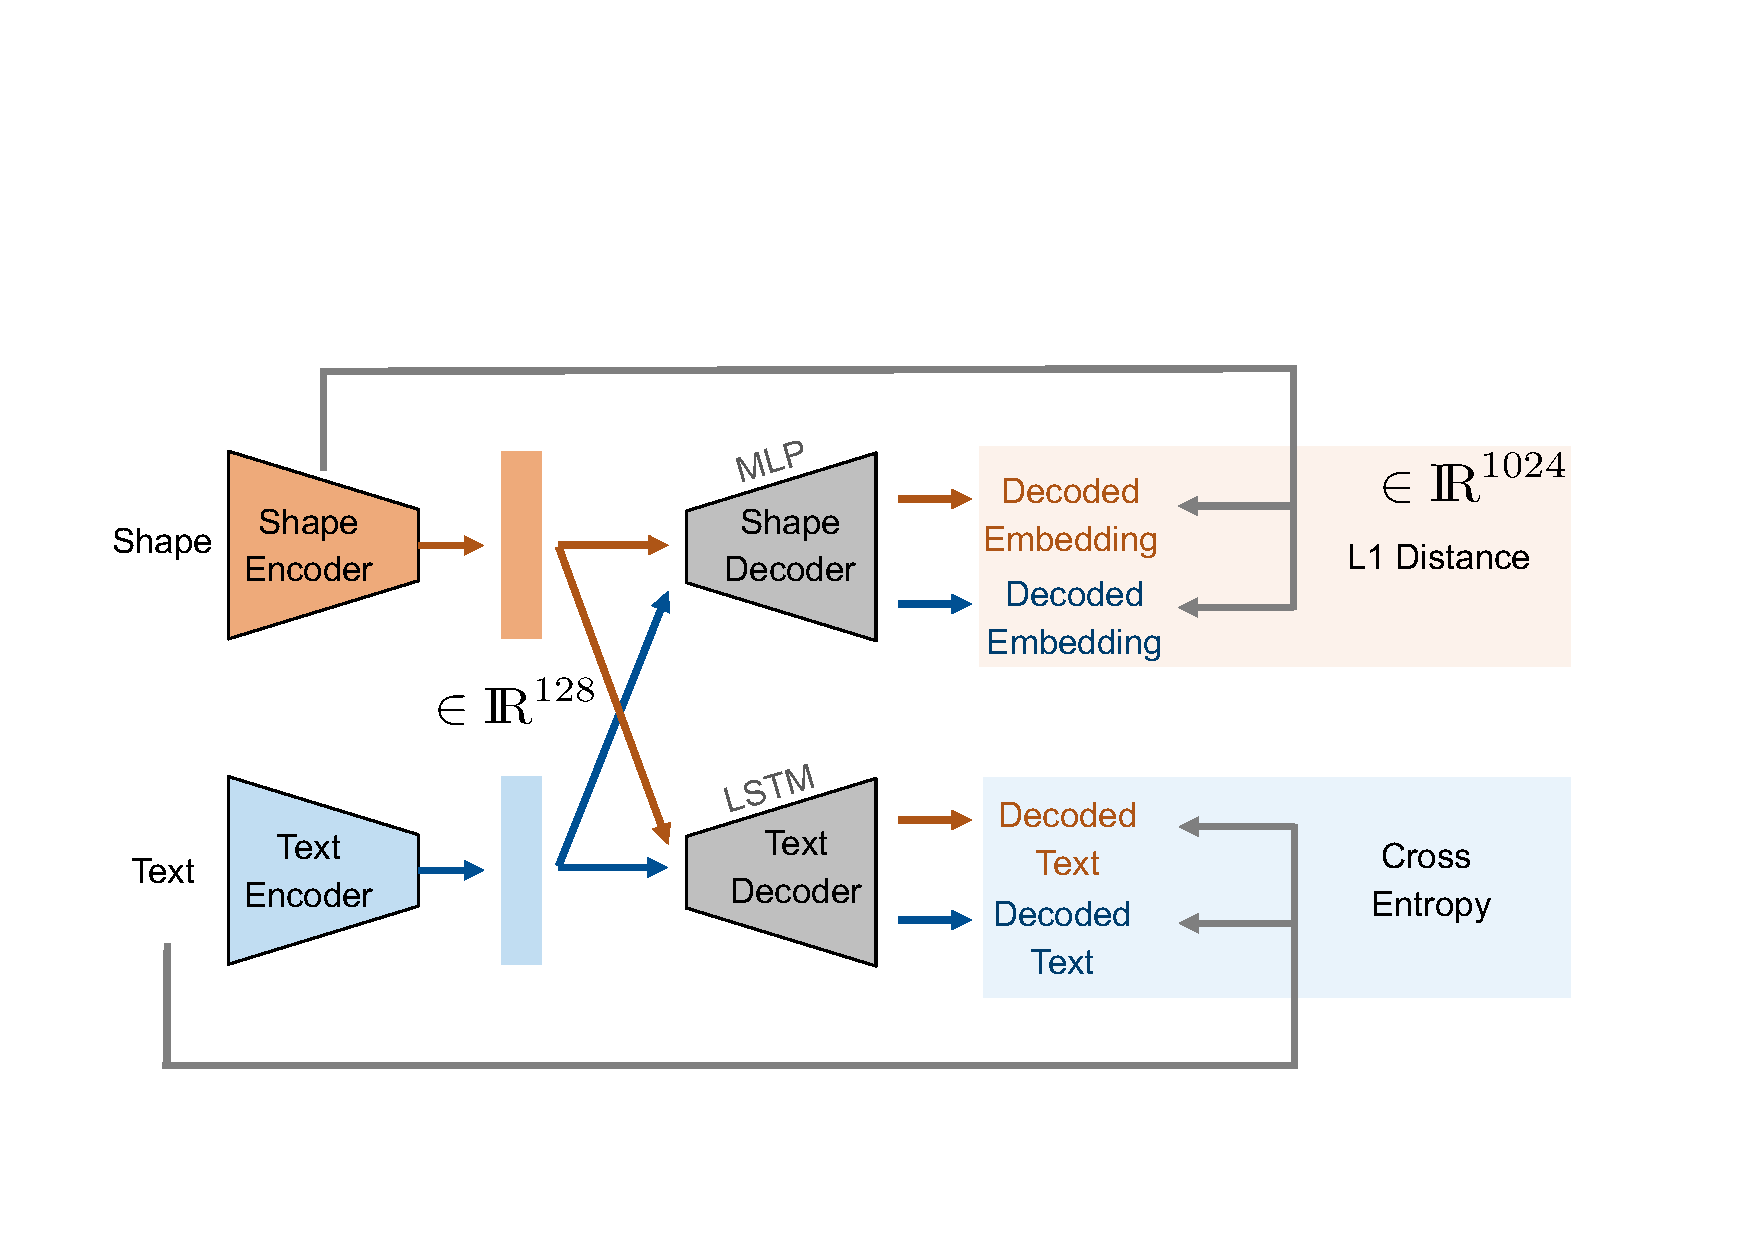
\includegraphics[width=0.8\linewidth]{fig4.pdf}
	\caption[]{The autoencoder structure of our Siamese network consisting of two encoders and two decoders}
	\label{fig:autoencoder}
\end{figure}
The shape decoder is a standard multilayer perceptron (MLP) projecting both shape and text embeddings up into a space of $\mathbb{R}^{1024}$. The up-projected embeddings are compared to an intermediate layer of PointNet++ with the same dimension using the L1 distance. The text decoder is similar to the encoder a two-layer LSTM which is initialized with an embedding vector as hidden state. Therefore, the LSTM is using the embeddings as context and is trained by a teacher forcing approach. That is a stable and fast method to train a recurrent neural network where at each time step the ground truth is feed as input into the network instead of using the predicted output of the previous time step.

A important aspect of our new network for better capturing the cross-modality is the crossed up-projection of the embedding vectors. So additionally to capturing cross-modal relations with the triplet loss, a text embedding is used to create a shape of the same instance and a shape embedding is used to create a text description of an instance. This approach hereby extends the standard autoencoder structure of projecting into a low-dimensional bottle neck layer and afterwards projecting up into the original space and trying to minimize the reconstruction error.

\section{Experiments and Results}
\begin{table}[t]
	\resizebox{\linewidth}{!}{\begin{tabular}{c c c c}
			\textbf{Model} & \textbf{RR@1} & \textbf{RR@5} & \textbf{NDCG@5} \\ \hline \hline
			Random & 0.11 & 0.35 & 0.23 \\ 
			Text2Shape [1] & 0.40 & 2.37 & 1.35 \\ \hline 
			Baseline & 1.14 & 6.00 & 3.51\\ 
			Autoencoder & \textbf{1.82} & \textbf{7.04} & \textbf{4.40} \\ \hline
			
	\end{tabular}}
	\label{tab:tab1}
	\caption{Comparison of the baseline model architecture to the autoencoder structure on the chairs and tables dataset using the recall rate @ k and normalized discounted cumulative gain
		@ k
	}
\end{table}
\begin{table}[t]
	\resizebox{\linewidth}{!}{\begin{tabular}{c c c c}
			\textbf{Model} & \textbf{RR@1} & \textbf{RR@5} & \textbf{NDCG@5} \\ \hline \hline
			Random & 0.08 & 0.39 & 0.23 \\ \hline
			Baseline & 3.13 & 11.98 & 7.50\\ 
			Autoencoder & \textbf{3.64} & \textbf{13.45} & \textbf{8.53} \\ \hline
	\end{tabular}}
	\label{tab:tab2}
	\caption{Comparison of the baseline model architecture to the autoencoder structure on 13 classes of the ShapeNetCore dataset with even distribution of 100 test samples per class using the recall rate @ k and normalized discounted cumulative gain
		@ k
	}
\end{table}
In this section we are presenting the qualitative and quantitative results of our network in both the baseline and autoencoder setting. For qualitative evaluation we implemented a retrieval function, were the user inputs a natural language text query and the database is searched for the best five retrievals. In that process, the network performs a forward path on the input sentence and searches in the embedding space for the five nearest neighboring shapes. Some exemplary results for the retrieval are shown in \autoref{fig:retrieval}. Our network can differentiate the input sentence and retrieve the correct kind of object and also works on attribute level, as can be see by comparing the search query for circle and glass top table.
\begin{figure}[t]%[!htbp]
	\centering
	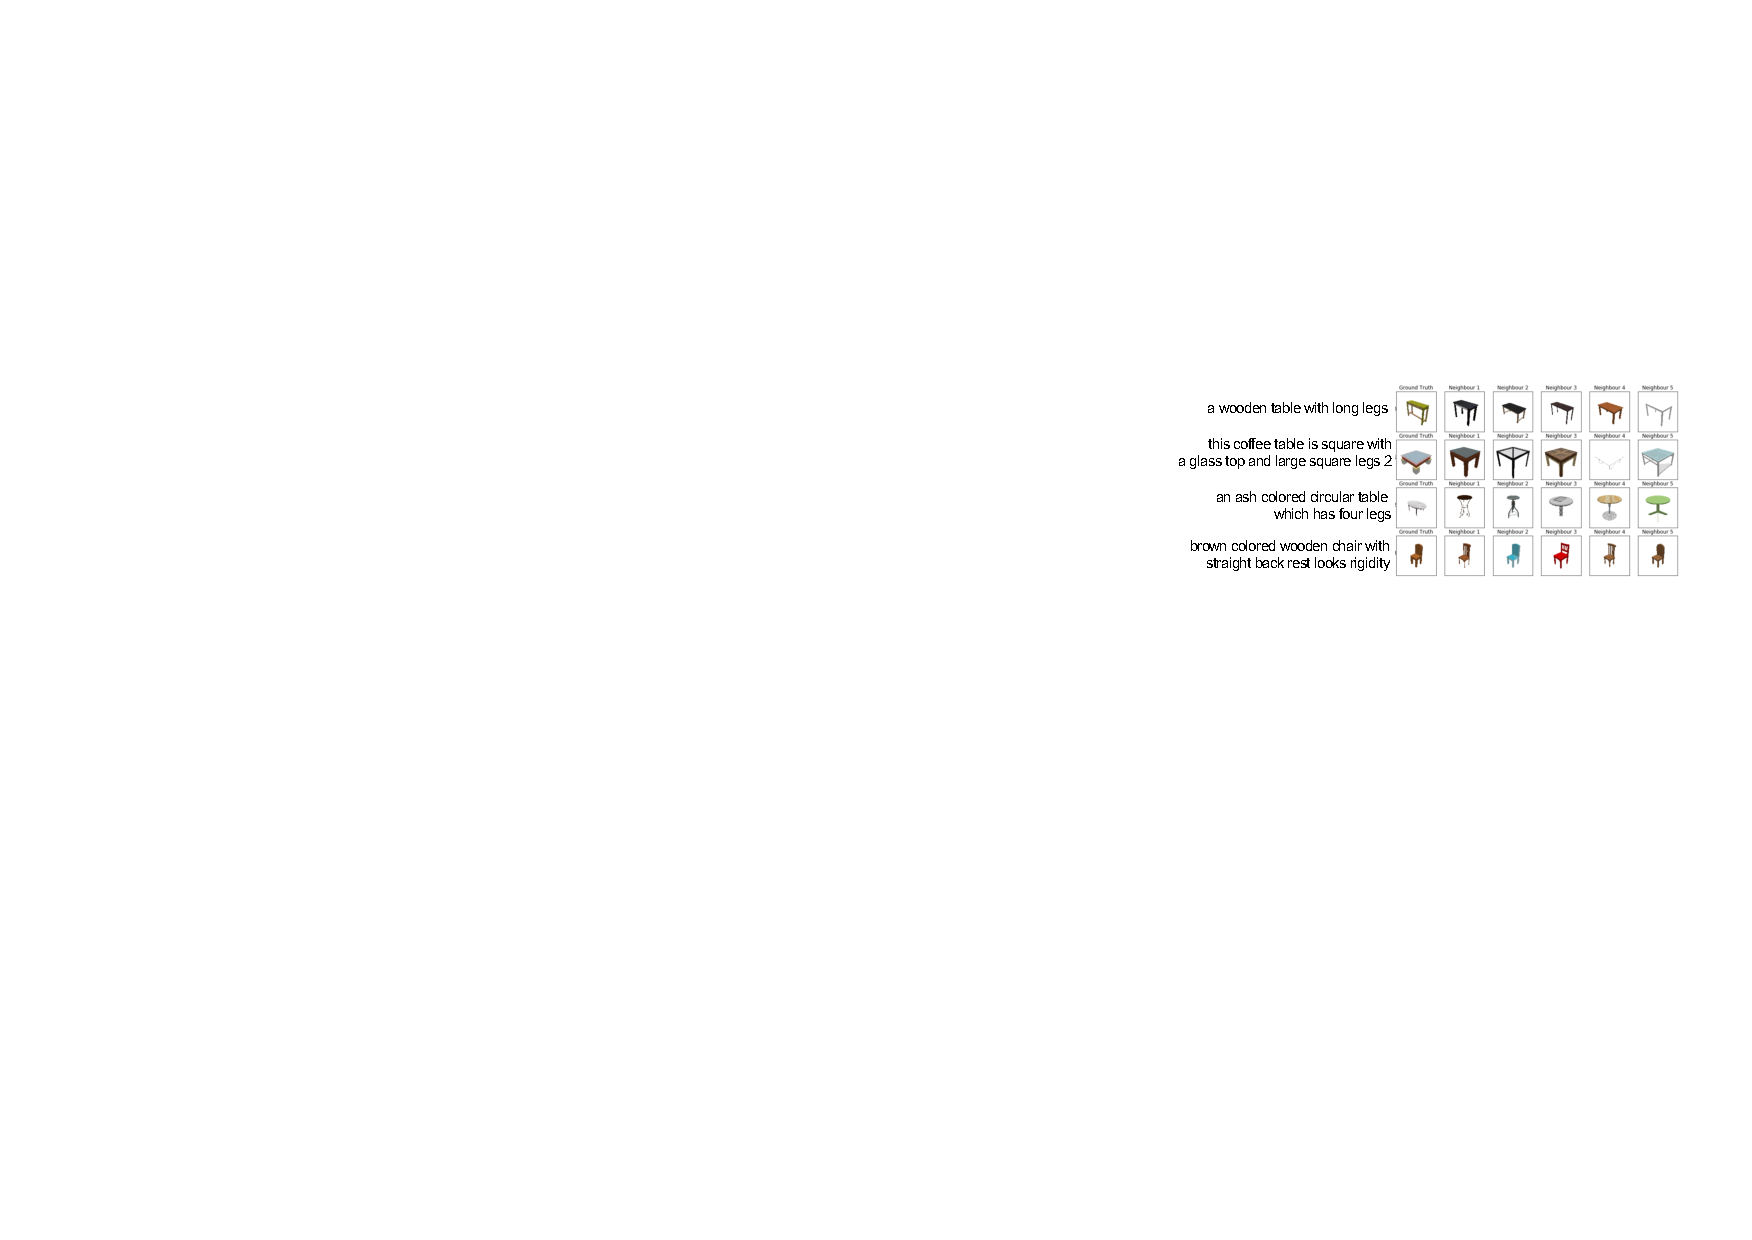
\includegraphics[width=1\linewidth]{fig5.pdf}
	\caption[]{Retrieval results for five different input text queries}
	\label{fig:retrieval}
\end{figure}

For quantitative evaluation we use the recall rate RR@k and the normalized discounted cumulative gain NDCG@k \cite{J_rvelin2002ndcg}. The recall rate RR@5 indicated, that for a input text the database is searched for the five nearest neighbors and if among those five the corresponding ground truth shape is obtained, the retrieval was successful. NDCG involves a discount function over the rank while RR@k uniformly weights all positions. This evaluation is performed on two different datasets which were formed from the ShapeNetCore dataset. First, we train and test both model settings on the subset of only chairs and tables. In total there are  12,100 training samples and 1,514 validation and test samples. The retrieval measures for this dataset are shown in \autoref{tab:tab1} and indicate a very good performance of our method. The baseline methods on point clouds outperforms the state of the art voxel-based approach and by applying the autoencoder structure a further small improvement could be reached. The second dataset we train and evaluate on contains 13 classes from ShapeNetCore and within each class all contained instances except for 100 validation and test samples. This lead to 25,210 training samples, which are not uniformly distributed, and 100 test samples per class. The results are depicted in \autoref{tab:tab2} and show still better performance measures than for just the chairs and tables.

\section{Conclusion}

{\small
\bibliographystyle{ieee_fullname}
\bibliography{3d_retrieval}
}

\end{document}
